\documentclass[10pt, a4paper, twocolumn]{article} 
\usepackage[english]{babel}
\usepackage{listings}
\usepackage{microtype}
\usepackage{amsmath,amsfonts,amsthm}
\usepackage[svgnames]{xcolor}
\usepackage[hang, small, labelfont=bf, up, textfont=it]{caption} 
\usepackage{booktabs}
\usepackage{lastpage}
\usepackage{graphicx}
\usepackage{enumitem}
\setlist{noitemsep}
\usepackage{sectsty}
\allsectionsfont{\usefont{OT1}{phv}{b}{n}}
\usepackage{geometry}
\geometry{
	top=1cm,
	bottom=1.5cm, 
	left=2cm,
	right=2cm,
	includehead, 
	includefoot
}
\setlength{\columnsep}{7mm}
\usepackage[T1]{fontenc} 
\usepackage[utf8]{inputenc} 
\usepackage{XCharter}
\usepackage{fancyhdr} 
\pagestyle{fancy} 
\renewcommand{\headrulewidth}{0.0pt}
\renewcommand{\footrulewidth}{0.4pt} 
\renewcommand{\sectionmark}[1]{\markboth{#1}{}} 
\lhead{} 
\chead{\textit{\thetitle}} 
\rhead{} 
\lfoot{} 
\cfoot{} 
\rfoot{\footnotesize Page \thepage\ of \pageref{LastPage}}
\fancypagestyle{firstpage}{ 
	\fancyhf{}
	\renewcommand{\footrulewidth}{0pt} 
}
\newcommand{\authorstyle}[1]{{\large\usefont{OT1}{phv}{b}{n}\color{DarkRed}#1}}
\newcommand{\institution}[1]{{\footnotesize\usefont{OT1}{phv}{m}{sl}\color{Black}#1}}
\usepackage{titling} 
\newcommand{\HorRule}{\color{DarkGoldenrod}\rule{\linewidth}{1pt}}
\pretitle{
	\vspace{-30pt} 
	\HorRule\vspace{10pt} 
	\fontsize{32}{36}\usefont{OT1}{phv}{b}{n}\selectfont 
	\color{DarkRed} 
}
\posttitle{\par\vskip 15pt} 
\preauthor{} 
\postauthor{ 
	\vspace{10pt} 
	\par\HorRule 
	\vspace{20pt} 
}
\usepackage{lettrine}
\usepackage{fix-cm}	
\newcommand{\initial}[1]{
	\lettrine[lines=3,findent=4pt,nindent=0pt]{
		\color{DarkGoldenrod}
		{#1}
	}{}
}
\usepackage{xstring}
\newcommand{\lettrineabstract}[1]{
	\StrLeft{#1}{1}[\firstletter] 
	\initial{\firstletter}\textbf{\StrGobbleLeft{#1}{1}}
}
\usepackage[backend=bibtex,style=authoryear,natbib=true]{biblatex}
\addbibresource{example.bib} 
\usepackage[autostyle=true]{csquotes}
 % Specifies the document structure and loads requires packages

\title{Implementando OpenGL con Oculus Rift SDK}

\author{
	\authorstyle{Jaime Margolin\textsuperscript{1}, Daniel Monzalalala\textsuperscript{1} and Juan Carlos León\textsuperscript{1}} % Authors
	\newline\newline 
	\textsuperscript{1}\institution{Instituto de Estudios Superiores del Tecnológico de Monterrey Campus Santa Fe}\\  }

\date{\today} 
\begin{document}

\maketitle 

\thispagestyle{firstpage} % Apply the page style for the first page (no headers and footers)

%----------------------------------------------------------------------------------------
%	ABSTRACT
%----------------------------------------------------------------------------------------

\lettrineabstract{El propósito del paper esta enfocado en dar una nueva perspectiva de como se puede incluir el uso de básicas y viejas funciones de OpenGL con la tecnología más sofisticada y moderna como lo es el SDK de Oculus y las librerías que utiliza esta última, y como estas tecnologías pueden ir de1 la mano para crear nuevas y mejores soluciones en el campo de las gráficas computacionales. Para esto se utilizaron librerías de modelos que el mismo SDK provee, logrando así una conjunción más armónica para el resultado final. Este paper ayudará a todos aquellos que en su momento quieran explorar el mundo de "VR" y quieran implementarlo de manera fácil y que quieran utilizar OpenGL envez del estandar para VR de DirectX.}

%----------------------------------------------------------------------------------------
%	ARTICLE CONTENTS
%----------------------------------------------------------------------------------------

\section{Introducción}

En la actualidad, hay campos que han surgido dentro del desarrollo de las tecnologías computacionales, siendo la Realidad Virtual uno de los que parece tener más futuro, el poder simular ambientes completos y poder hacer que el mismo usuario puede estar inmerso en el mismo, haciendole pensar que esta en un ambiente como en el que esta acostumbrado a interactuar.

Ahora una de las prácticas que se ha vuelto de las más comúnes es el uso de Oculus Rift, el cual es un dispositivo que puede simular en forma 3D ambiantes, los cuales son controlados por el mismo dispositivo, este dispositivo es un tanto parecido a unos lentes, haciendo asi que la combinacion entre los lentes y un buen equipo de sonido portátil (audífonos) ó estático (bocinas) puedan hacer que el usuario se sienta en el lugar que se esta simulando, un lugar que puede ver ante sus propios ojos e inclusive en algunas ocasiones y con algunos otros aditamentos, hacer que se pueda interactuar de manera \textbf{\textit{"normal"}}.



%----------------------------------------------------------------------------------------
\section{Trabajo Previo}

El trabajo previo en el campo del Oculus SDK esta desarrollado en DirectX y los mismos desarrolladores del SDK recomiendan utilizarla. Encontramos muy poco realizado con OpenGL en el campo del oculus rift....


\subsection{Augmented Reality Under Water [2]}
A diferencia de lo que se puede pensar, este paper trata de cómo se hizo para que se utilizará el Oculus debajo de una alberca, en donde dependiendo de si había o no agua, hacia el render de ciertas cosas, en un inicio, la idea fue mostrar algo así como un acuario, en donde aparecían peces, arena, algas y otros elementos que se encuentran normalmente en el mar. Desde cómo organizar todos los componentes necesarios para que el usuario pudiera tener la mejor de las experiencias.

\subsection{Egocentric Distance Perception in the Oculus Rift (DK2)[1]}
Este paper habla acerca de la percepción del usuario cuando utiliza el Oculus Rift, habla de cómo se puede lograr que el usuario pueda tener cierta percepción “realista” para que el usuario sienta que en realidad está dentro de la realidad aumentada, los resultados arrojaron fórmulas y técnicas de modelación para lograr esto.

\section{Desarrollo}
Nosotros intentamos crear una pecera  con distintos animales marinos utilisando el SDK del oculus rift  \textbf{DK2} para OpenGL. Por las funciones que el SDK para OpenGL nos ofrecía, así que optamos por realizar este acuario con \textit{pixel art} que es una especie de representación de los objetos en formas más cuadradas al estilo de los videojeugos de \textbf{8 bit}.

El desarrollo consistió en tomar como base el (único) proyecto ejemplo que tenia el SDK en OpenGL. Este ejemplo consistía de un pequeño cuarto con una mesa una silla un cubo que gira y un mueble de pared. Lo que se realizó fue investigar como estaba compuesto el código. Se encontró la función:
\lstset{language=C++,
                keywordstyle=\color{blue},
                stringstyle=\color{red},
                commentstyle=\color{green},
                morecomment=[l][\color{magenta}]{\#}
}
\begin{lstlisting}
AddSolidColorBox(float x1, float y1,
 float z1, float x2, float y2, 
 float z2, DWORD c)
\end{lstlisting}
que lo que hace es agregar una "caja a la escena". esta función recibe como parámetros la x, y, z iniciales , la x, y, z finales y el color de la caja en hexadecimal.

\subsection{Armado del mundo}
\subsubsection{La pecera}
El mundo consta de 4 paredes 1 piso y 1 techo. estos forman la pecera en la que los distintos animales marinos estaran nadando.
Cada una de las paredes y el techo son creados agregando un cubo con 2 de sus aldos grandes y el 3 muy pequeño para que asi se asemeje a una pared delgada. El piso es creado de igual forma. por ultimo los colores que se le asiganaron a las paredes y al techo fue el mismo tono de azul, esto se eligio para lograr un efecto de continuidad. este efecto evita que se peuda diferenciar el momento en el que empiesa una pared y otra y donde conectan con el techo, asi dando un mayor sentido de profundidad.
Al piso se le asigno un color amarillento para que se parezca a la arena del mar. 
se intento agregar alguna de las texturas que ya estan incluidas en el SDK al piso para hcerlo parecer mas real pero las texturas del SDK daban la impresion de ser mosaicos y esto restaba un poco de realismo a la escena.  

\subsubsection{Las algas}
Las algas constan de un tallo de altura semi aleatoria. La altura del tallo es de 0.8 mas un número aleatorio que va del $0.0$ al $0.7$ esto nos da una altura alteatoria de $0.8$ a $1.5$. También se agregan hojas a la algas. Las hojas constan de 4 cubos pequeños acomodados en diagonal a partir del tallo. A una altura aleatoria de $0.2$ a $0.3$. cada alga puede tener de 0 a 4 hojas y esto también se decide de forma aleatoria. Y por último la posición de las hojas también se decide de forma aleatoria. Esto significa que sin importar la cantidad de algas que se agreguen a la escena habrá una gran variadad de algas con apariencias ligeramente diferentes para darle un toque de mayor realismo a la pecera.

\subsubsection{Los peces}
Los peces estan compuestos por 3 elementos principales: el cuerpo, la cara, las aletas. el cuerpo del pez consiste de un cubo grade de $1*1*1$. Los demas elementos del pez van "pegados" al cuerpo. la cara del pez esta compuesta por una boca que es un rectángulo pequeño en el centro en el eje $X$ y a $1/3$ del eje $Y$ del lado frontal del cubo, los ojos son 2 cuadros pequeños y negros a $1/3$ y $2/3$ del eje $X$ y a $2/3$ del eje $Y$ del lado frontal del pez. 

Las aletas entan divididas de la siguiente forma: 2 aletas laterales, 1 aleta dorsal y 1 aleta trasera. Las aletas laterales constan de 2 rectángulos delgados. Uno más pequeño que esta directamente pegado al pez y otro más grande conectado al primero. Los colores de las aletas son diferentes al del cuerpo del pez y cada uno de los rectángulos tiene su propio color.

La aleta dorsal esta compuesta de un rectángulo horizontal largo y de otro más corto. Esta aleta se colocó en la parte superior del pez. Ambos rectángulos están directamente pegados al cuerpo del pez, primero el rectangulo grande seguido del chico. Los colores son los mismos que los de las aletas laterales. 

La aleta trasera, o cola, esta compuesta de 3 rectangulos de tamaño creciente y ancho decreciente. El más pequeño y grueso esta pegado al pez mientras que el más grande y delgado es el más alejado. el primer rectángulo va pegado al pez de forma vertical, el segundo va pegado a este y el tercero al segundo. Los colores de estos rectángulos son, el primero y tercero tienen el color del primer rectángulo de las aletas laterales y el 2° rectángulo tiene el color del segundo rectángulo de las aletas laterales.

\subsubsection{Tiburón}
El tiburón sigue la misma lógica de contrucción que los peces, únicamente se modificó el largo del cuerpo que para el tiburón es de $1*1*3$ y el grosor de las aletas, estas se hicieron más gruesas para darle un toque de realismo. También se adecuo el posisionamiento de las aletas para que se mantuviera la proporcion del cuerpo. El tiburón es completamente negro con tonos grises en las aletas y ojos blancos.

\subsubsection{Erizo}
Para darle variedad a la vida marina en la pecera se decidió agregar un erizo de mar. El erizo tiene un cuerpo cuadrado de $0.5*0.5*0.5$ y 5 espinas. su cuerpo y espinas son de color gris. las espinas fueron creadas de forma en que todas estuvieran distibuidas por el cuepro del erizo y tuvieran longitudes ligeramente diferentes para dar un toque de realismo.

\subsection{Construccion del mundo}
Con todos los elementos del mundo armados se tienen que agregar a la escena. Para dar un toque de realismo se decidió que las posiciones de los peces como de las algas deberían ser aleatorias. 

\subsubsection{Tiburón y Erizo}
Por sus caracteristicas y funciones dentro de la escena se opto por dejar al tiburón y al erizo en una posición de inicio fijas.

\subsubsection{Algas}
Las algas de decidió que debería de tener un posición aleatoria dentro de la pecera para dar un toque de realismo. cada vez que se corre el programa las algas se crearán en lugares distintos. Como se agrega una gran cantidad de algas a la escena el darles una posición aleatoria ayuda a distribuirlas. Las algas se crean en un rango de $-10$ a $10$ en $X$ y de $-20$ a $20$ en $Z$, esto para abarcar la totalidad de la pecera.

\subsubsection{Peces}
La posición inicial de los peces también es aleatoria para dar un \textbf{toque de realismo}. Pero para mantenerlo visualmente estético se decidio que la altura a la que nadan los peces seria pre definida, asi se evita que los peces pasen unos sobre otros. la altura mas baja es para los que nada en linea vertical (recorrido largo en el rectángulo que forma la pecera) mientras que los que nadan mas alto son los que recorren la pecera de forma horizontal (recorrido corto en el rectángulo que forma la pecera).

\subsection{Animaciones}
Para dar un toque de realismo se animaron todos los animales marinos de la escena. Las animaciones fueron de las partes más retadoras ya que se trato de mantener una animación congruente con el \textbf{pixel art} de la escena pero a la vez de hacerlo parecido a la realidad para mentener el toque de realismo que se le esta intentando dar al proyecto.

\subsubsection{Erizo}
El erizo es el animal con el movimiento más siemple. Se mueve siempre en un círculo alrededor del centro ($x/2,y/2$) de la pecera, también es el mas rápido de todos los animales y el único que se mueve por al ras de piso.

\subsubsection{Tiburón}
A petición del profesor \textit{"Estaría padre que agreguen un tiburón asi, como que vaya como acechando a los otros peces"} se agregó el tiburón y la animación tenia que ir de acuerdo a dicha petición. Se opto por el movimiento en forma de \textit{8 extendido}, para que entre y salga de la escena como si estuviera acechando a los peces. El tiburón es el mas lento para dar un toque de realismo al depredador acechando.

 \subsubsection{Peces}
Los peces son los animales con mas movimientos. Para dar un toque de realismo se les programo un movimiento hacia el frente mientras que tienen un movimiento ondulatorio ya sea hacia arriba y abajo o de derecha a izquierda. 
 
Ademas de tener una posicion de origen aleatoria los peces tienen movimiento aleatorio, la velocidad con la que avanzan hacia el frente es aleatoria entre $0.22$ a $0.44$. esto hace que los peces se muevan a diferentes velocidades y da un toque de realismo a la escena.

Con fines demostrativos para la exposicion se decidio fijar el movimiento ondulatorio de los peces de la siguiente forma. lo que se mueven de forma vertical ondulan de arriba abajo mientras que lo que de mueve en forma horizontal ondulan de derecha a izquierda. 

\section{Complicaciones}
\subsection{Figuras}
El primer problema con el que se encontro es que el SDK para el oculus únicamente tiene una figura, \textbf{el cubo}, por lo que la primera restriccion y la mas compleja fue el tener que armar todo con subos. Tambien la funcion que crea los cubos recibe como parametros la XYZ inicial y final, a diferencia de las funciones basicas que se vieron en clase que reciben unicamente el tamaño del cubo (y este es creado en la posición en la que se encuentra GL en ese momento). Por lo que todas las posiciones y movimientos de la escena fueron calculados por nosotros. 

Para lograr las distintas figuras de la pecera se hicieron muchos cálculos para lograr modificar los cubos a que fueran cuadrados y rectángulos que se pudiera utilizar en el proyecto. Además del cálculo que hicimos para posicionarlos unos con respecto de otros.

\subsection{OpenGL SDK vs lo visto en clase}
Encontramos diferencias substnaciales entre lo que se usa en el SDK del oculus y lo que se vio en clase. Aquí enlistaremos las que nos causaron el mayor número de problemas. \begin{itemize}
\item GL main loop - En este proyecto no hay un main loop que se parezca al main loop de GL. La función del main loop se encarga de hacer un trabajo similar, pero no acepta ninguna de las funciones de GL dentro.
\item GL init - No hay una función de init como en GL.
\item Funciones de GL - en el SDK del oculus no sirven ninguna de las siguientes funciones que se vieron en clase
\begin{itemize}
\item push matrix
\item pop matrix
\item rotate
\item scale 
\item translate
\item curvas 
\item superficies
\end{itemize}
\item Luz - La luz como se vio en clase se agrega 1 (o varias) fuente(s) de luz a la escena la cual interactúa con los materiales de los objetos para ser reflejada. En el proyecto no hay ninguna fuente de luz, si no que cada objeto tiene su propio color, que de cierta forma es la luz que este objeto irradia, pero sin afectar a las demás o reflejarse en otros objetos.
\end{itemize}

\subsection{.OBJ's}
Se intento cargar archivos \textbf{.OBJ} de muchas maneras y ninugna permitio cargarlos. se probaron varias librerías y métodos entre los que destacan: glm (visto en clase) y assimp.

Inclusive se intento cargar los archivos con Directx y tampoco se logro el objetivo.

\section{Resultados}
El proyecto se concluyó en tiempo y forma, con todas las peticiones \textbf{extras} que el profesor expresó, dando así el siguiente resultado:

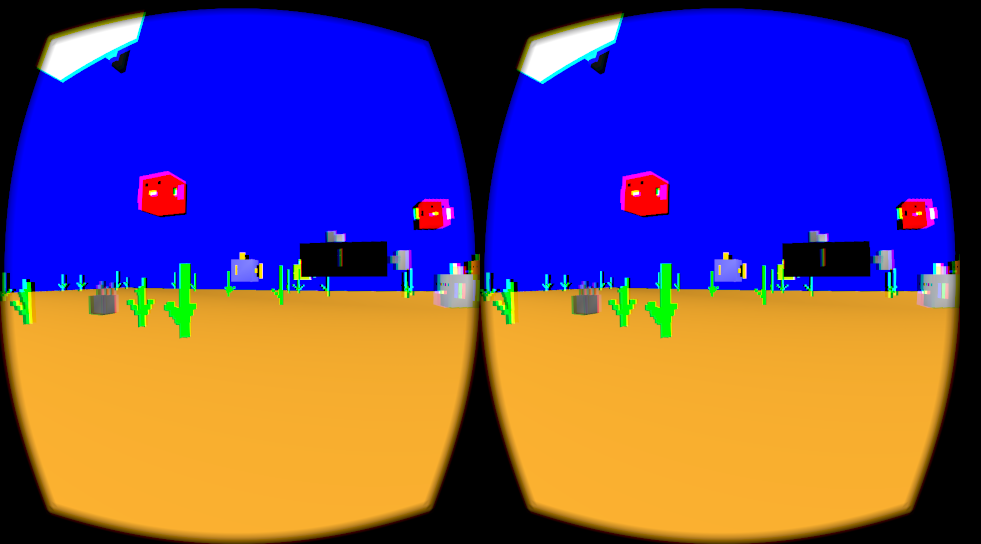
\includegraphics[width=\linewidth]{screen6.PNG}

Dando así por terminado el primer acercamiento de nuestra parte con el Oculus Rift y el uso del SDK con librerías open source como lo es OpenGL.

\section{Trabajo Futuro}
Se espera que en un futuro, sigamos utilizando el SDK de Oculus con librerías nuevas y más actualizadas para llegar a tener una mejor versión final de este proyecto, donde podamos involucrar conocimientos más avanzados como el cargar OBJ's, texturas e inclusive poder llevarlo a un campo más real para que el usuario crea que está en un acuario sin necesidad de tener que ir a uno, un ejemplo de como sería este proyecto sería:

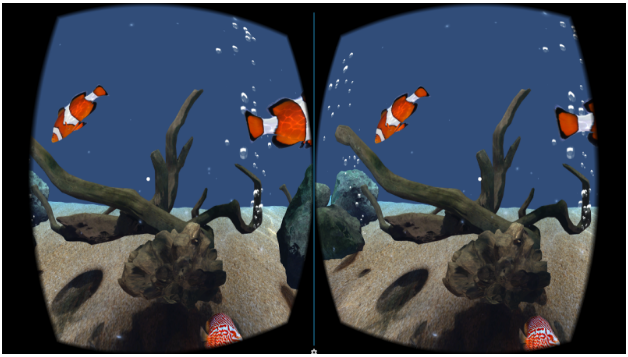
\includegraphics[width=\linewidth]{peces.png}

\section{Conclusiones}
El uso de OpenGL puede ser muy eficiente si se conoce la tecnología y si la plataforma en la que se quiere aplicar esta enfocada a esto, también podemos darnos cuenta como hay librerías que ya contienen funcionamiento de OpenGL sin necesidad de programarlo al más bajo nivel.

Durante el proceso el aprendizaje fue bueno, ya que tuvimos que aprender a crear cosas que no se conocían, por lo cual el tiempo de investigación fue largo y tardado pero rindió fruto, ya que el proyecto se logró de muy buena manera y con peticiones más allá de las que se habían especificado en el planteamiento del mismo, así que el equipo salió con muy buen aprendizaje orientado a los ambientes 3D.

Fue un reto interesante, ya que la complejidad era mayor que los demás proyectos, porque es tecnología no vista en clase así como un mundo con interacción 3D, que se presentaron y por esa razón fue más divertido, sin duda alguna se volvería a trabajar con el Oculus Rifft pero utilizando DirectX ya que el soporte para este último es mejor y más orientado a la plataforma.

%----------------------------------------------------------------------------------------
%	BIBLIOGRAPHY
%----------------------------------------------------------------------------------------

\begin{thebibliography}{9}
\bibitem{paper1}
Egocentric Distance Perception in the Oculus Rift (DK2)
\\\texttt{https://goo.gl/R0zcmS}

\bibitem{paper2}
Augmented Reality Under Water
\\\texttt{http://bit.ly/2qkAGHU}

\bibitem{oculus sdk}
Oculus SDK
\\\texttt{https://developer.oculus.com/downloads/}
\end{thebibliography}

%----------------------------------------------------------------------------------------

\end{document}
